\documentclass[11pt,titlepage]{article}
\usepackage[margin=1in]{geometry}
\usepackage{amsmath,graphicx, url, float, multicol}
\floatstyle{boxed}
\restylefloat{figure}

\title{Collabrador: a collaborative peer-to-peer text editor}
\newcommand{\name}[2]{#1 \\[-4pt] {\small \url{#2}} \\[4pt]}
\author{
  \name{Jacob Hurwitz}{jhurwitz@mit.edu}
  \name{Colleen Josephson}{cjoseph@mit.edu}
  \name{David Lawrence}{dlaw@mit.edu}}
\date{
  May 10, 2012 \\ \small
  R07 and R09 with Nir Shavit}
\begin{document}
\maketitle

\section{Introduction}

Collabrador is a peer-to-peer text editor that lets multiple users
collaborate on a document. Users can edit a document while online or
offline, although they cannot view each other's changes until they
join a (possibly ad-hoc) network and synchronize.  In addition to
storing the text of a document, Collabrador logs each user's edits as
individual insert, delete, and move operations.  When users make
distinct changes to a document, the branches can be merged by
replaying the changes made by one user atop the changes made by
another user.  This technique is known as the operational transform
and is the basis for all major collaborative editors.

\section{Design}

\subsection{System architecture}

On each computer, Collabrador consists of a \emph{text editor} and a
\emph{checkpoint database}. In addition to storing the text,
Collabrador's text editor saves a description of the
\emph{operations} performed by the user. These operations are
inserting a character at a given position (\emph{insert}), deleting
a character at a given position (\emph{delete}), and using cut/paste
to move a block of text from one position to another (\emph{move});
collectively, these operations form an \emph{operational
  transformation} describing how the user modified the initial
document. When the user clicks the ``save'' button, Collabrador
creates a \emph{checkpoint} containing this operational
transformation and saves it into the local \emph{checkpoint
  database} \cite{ot}.

To be more specific, Collabrador stores a checkpoint database
consisting of \emph{checkpoint objects}. A checkpoint object is a data structure
encapsulating the details of the operational transformation performed
by that edit, the hashes of the edit's parent or parents, the hashes
of the edit's children, the hash of the unique checkpoint to be used
as the base of the operational transformation, and the \emph{user
  visibility list}, which is just the list of users that have locally
stored this checkpoint. Checkpoint objects are keyed by the SHA-1 hash of
the object itself. For full implementation details, see
Section~\ref{sec:storage-dag}.  We will assume that SHA-1 has no collisions,
so two checkpoints will have the same hash if and only if they perform
the same changes to the same base from the same parents.

When the system consists of a single computer, the checkpoint database
is just a linear progression of checkpoints. Adding in multiple
computers, a hypothetical central server keeping track of edits on all
computers would model the checkpoint database as a directed tree, with
a branching node occurring whenever two computers make distinct
edits. If two computers are allowed to synchronize with each other,
then branches of this tree can join together (creating nodes with two
parents instead of just one) and so the checkpoint database becomes a
directed acyclic graph (DAG) instead, where the nodes are checkpoint objects,
and the edges are OTs.  (For this reason, this paper
uses the terms \emph{checkpoint database} and \emph{DAG}
interchangeably.)  The challenge with Collabrador is to maintain this
DAG in a distributed fashion because there is no central
server. Collabrador's solution is %for each user to store in its local
%checkpoint database only the portion of the graph that it knows about while 
a synchronization process in the background that lets users
constantly communicate with each other to share and exchange parts of
the graph. Collabrador operates on top of TCP/IP to ensure reliable and
in-order packet delivery. 

The checkpoint database can be in two states. At most times, a user's 
checkpoint database will be a graph with only a single leaf node, 
representing the most recent checkpoint created by the user. 
A database with just one leaf node is in the \emph{merged}
state. When synchronizing with another user, that user's checkpoint
objects will be copied into the local checkpoint database, causing the
graph to have two leaf nodes. A database with two leaf nodes is in the
\emph{unmerged} state. Then, as described in
Section~\ref{sec:merge}, the Collabrador merge algorithm will find the
least common ancestor of these leaves, merge the two edits into a
single checkpoint, and then save this checkpoint into the database as
a node with two parents and an operational transformation relative to
the least common ancestor.

\subsubsection{Storage of the DAG}
\label{sec:storage-dag}

The system used by clients to store the DAG of document versions must
meet performance and reliability requirements.

The performance requirements are easily addressed by having each node
store pointers to its children, parents, and the lowest common
ancestor of its parents.  Since nodes are named by hash, we also
maintain an index table containing pointers to nodes by hash.
Finally, we keep pointers to all current leaf nodes (usually one, but
sometimes two), and the original common ancestor for the document.
Using this structure, we may perform all relevant graph traversals in
constant time per node.

To meet our reliability (particularly atomicity) requirements, we
store the DAG in a database that is designed specifically to provide
fault-tolerance guarantees.  One such candidate is PostgreSQL
\cite{postgres}.

\subsection{Sync algorithm}

\emph{Synchronization} is a process which causes two computers with 
unique checkpoint databases to converge to a single checkpoint database. 
Each machine must begin and end with a checkpoint database in the merged 
state. The computer that initiates the synchronization
process is called the \emph{initiator}, and the other computer is
called the \emph{provider}. At a high level, the synchronization
process performs three steps:
\begin{enumerate}
\item The provider sends its checkpoint database to the initiator.
\item The initiator, which is now unmerged, locally performs the merge
  algorithm described in Section~\ref{sec:merge}.
\item The initiator sends its (now merged) checkpoint database to the
  provider.
\end{enumerate}
One possible implementation of the synchronization process would be to
have the provider send its entire checkpoint database to the initiator
in the first step. However, it is usually the case that most of the
provider's database is already known to the initiator. To minimize the
amount of communication required, the provider only needs to send the
checkpoint objects it has that the initiator does not have. The process 
for discovering which objects the initiator does not have is described 
below.

Let $I$ be the leaf node of the initiator's database, let $P$ be the
leaf node of the provider's database, and let $C$ be any common
ancestor of $I$ and $P$. There is guaranteed to be at least one common
ancestor because, at the very least, the object representing the
initial blank document is necessarily an ancestor of all checkpoint
objects. Thus, the provider only needs to send the nodes ``between''
$C$ and $P$. To further minimize the amount of the database
transmitted, it's ideal for $C$ to be the \emph{least} common ancestor
of $I$ and $P$.

To find the least common ancestor in a distributed fashion, the
provider performs the following algorithm: It sends $P$'s hash to the
initiator and asks if this object was already in the initiator's
checkpoint database. If it was, then this step of the synchronization
process is complete. However, Collabrador also needs to update $P$'s
user visibility list to include both the initiator and the provider
(if they weren't already included). If $P$ was not already in the
initiator's database, then the initiator asks for the full checkpoint
object corresponding to $P$, and then the provider sends both this and
recusively sends the hashes of $P$'s parents using the same
process. This process will terminate upon reaching $C$. At this point,
the initiator has the provider's entire checkpoint database.

Next, the initiator performs the merge algorithm using this most
recently transmitted object $C$ as the common ancestor, and sets the
user visibility list of the resulting leaf node to contain only the
provider and the initiator. Finally, the initiator sends its entire
checkpoint database to the provider using the aforementioned process.

When there are more than two computers, Collabrador has them
synchronize in a pairwise fashion. The implementation of Collabrador
assumes that each user can query for the set of all users currently on
the network. Every computer has a background process that, at random
intervals, sends a request to another computer asking if it is willing
to synchronize.  The two conditions under which a computer will refuse
a request are if it is waiting for a response from any computer about
synchronizing (up to some time-out), or if it is currently
synchronizing. Syncronization also ocurrs when a user saves or initiates
a named checkpoint. When two computers agree to synchronize, the computer
that initiated the request will play the role of initiator and the
other computer will be the provider. When this process finishes, the
initiator will wait a random interval and then send a request to
the user currently on the network with the next-lowest IP address in a
round-robin process. After a quadratic number of pairwise
synchronizations, all computers in the network will converge on the
same checkpoint database.

Additionally, whenever two computers synchronize, they also exchange
their \emph{known user lists}. All users, whether online or offline,
are included. The purpose of this exchange is so that all users
collectively can determine the exact group membership, even if users
are dynamically joining the group. Collabrador does not, however,
support users dynamically leaving the group.

\subsection{Merge algorithm}
\label{sec:merge}

The merge algorithm is based on the operational transform (``OT''),
which is the conflict resolution technique used by all major
collaborative software (notably including Google Docs and
SubEthaEdit).  We model a single OT as a sequence of non-conflicting
``insert'', ``delete'', and ``move'' operations.  Note that every OT
defines a transformation on character indices (although this
transformation need not be injective or surjective), and all OTs are
invertible.  A full formal description of OTs is given in \cite{wave}.

OTs can interact in several ways, which are shown in
Figure~\ref{fig:ot}:
\begin{itemize}
\item Any number of OTs that are generated sequentially may be
  composed into a single OT representing the combined effect.  We can
  thereby express an OT that represents the transformation between any
  commit and its parent, regardless of how many steps the user took to
  effect this transformation.
\item We may use an OT, viewed as a transformation on character
  indices, to transform the indices of another OT.  This process will
  fail if and only if there are conflicting changes in the two OTs.
\item When two OTs are performed simultaneously, we may use one OT to
  transform the character indices of the second OT, and compose the
  result with the first OT.  This process is commutative when there
  are no conflicts.
\end{itemize}

When the merge algorithm takes over, the sync algorithm has copied
nodes between two merged DAGs, resulting in an unmerged DAG.  The sync
algorithm has also identified the lowest common ancestor of the two
leaves in the unmerged DAG.  We must merge these into a single
leaf---automatically if possible, but with user intervention if
necessary. Formally, given two OTs that take the same parent to
different children, we wish to generate a single OT that applies both
sets of changes to the parent in a logical way.

We simply follow the approach mentioned above: use one OT to transform
the character indices of the second OT, and compose the result with
the first OT.  Conflicting portions of the second OT are ignored and
flagged for manual user resolution.  (Following the New Jersey design
approach, we prohibit incorrect automatic merges, but allow
unnecessary manual merges if it makes the implementation substantially
simpler.)  When conflicting changes are identified, they are flagged
for manual resolution, but the algorithm continues to resolve
subsequent non-conflicting changes.  An example is shown in
Figure~\ref{fig:merge}.

\begin{figure}[h]
  \centering
  \begin{minipage}{\textwidth}
    \begin{multicols}{2}
      \setlength{\parskip}{-6pt}
      \subsubsection*{OT primitive operations}
      An OT is defined as a composition of the following primitive
      operations:
      \begin{eqnarray*}
        &insert(substring, index) \\
        &delete(start\_index, end\_index) \\
        &move(start\_index, end\_index, new\_loc)
      \end{eqnarray*}      
      \subsubsection*{Example strings}
      \begin{eqnarray*}
        A &=& \mathrm{^0i^1n^2s^3i^4d^5e^6\_^7o^8u^9t^{10}} \\
        B &=& \mathrm{^0o^1u^2t^3s^4i^5d^6e^7\_^8i^9n^{10}} \\
        C &=& \mathrm{^0o^1u^2t^3s^4i^5d^6e^7} \\
        D &=& \mathrm{^0i^1x^2n^3s^4i^5d^6e^7\_^8o^9u^{10}t^{11}}
      \end{eqnarray*}
      (Superscripts denote character indices.)
      \subsubsection*{String/OT relationships}
      \includegraphics[width=\columnwidth]{fig.pdf}
      \subsubsection*{Example OTs}
      \begin{eqnarray*}
        X &=& move(5, 8, 0) \circ move(0, 2, 10) \\
        Y &=& delete(7, 10) \\
        Z &=& insert(1, \mathrm{x})
      \end{eqnarray*}
      We have \(X(A) = B\), \(Y(B) = C\), and \(Z(A) = D\).  The
      complete diagram of relations is given in figure 
      \subsubsection*{Composition}
      The composition \(Y \circ X\) is performed in the obvious way,
      and we have \((Y \circ X)(A) = C\).
      \subsubsection*{Parallel composition}
      When two users perform diverging modifications (for example,
      \(X\) and \(Z\) to \(A\)), we merge them by transforming the
      transform.  For example:
      \begin{eqnarray*}
        X(Z) &=& insert(9, \mathrm{x}) \\
        Z(X) &=& move(5, 8, 0) \circ move(0, 3, 11)
      \end{eqnarray*}
      We would merge the users' changes as follows: \[(X(Z) \circ
      X)(A) = (Z(X) \circ Z)(A) = \mathrm{outside\_ixn}.\] This
      process is formally described in \cite{ot}.
      \subsection*{Merge conflict}
      The quantities \((Y \circ X)(Z)\) and \(Z(Y \circ X)\) are not
      defined.  Both transformations of indices fail because there are
      conflicting changes.
    \end{multicols}
  \end{minipage}
  \caption{Operational transform examples.}
  \label{fig:ot}
\end{figure}

\begin{figure}[h]
  \centering
  \begin{minipage}{\textwidth}
    \begin{multicols}{2}
      \subsubsection*{The scenario}
      Start with the document ``abc'', and consider the following OTs:
      \begin{eqnarray*}
        U &=& insert(3, \mathrm{z}) \circ insert(1, \mathrm{x}) \\
        V &=& insert(1, \mathrm{y}) \circ insert(2, \mathrm{z})
      \end{eqnarray*}
      So \(U(\mathrm{abc}) = \mathrm{axbzc}\) and \(V(\mathrm{abc}) =
      \mathrm{aybzc}\).  The user must manually resolve the``x'' vs
      ``y'' merge conflict, but ``z'' should be merged automatically.
      \subsubsection*{Merge difficulties}
      Both users have made the same change (inserting ``z''), so a
      merge conflict should not be generated for that character.  The
      users also made a conflicting change (``x'' vs ``y''), but one
      did so before inserting ``z'' and one did so after inserting
      ``z''.
      \subsubsection*{The merge}
      First we compute \(U(V)\). \(insert(1,\mathrm{x})\) transforms
      \(insert(2,\mathrm{z})\) to \(insert(3,\mathrm{z})\).  We
      attempt to apply the coordinate transformation of
      \(insert(1,\mathrm{x})\) to \(insert(1,\mathrm{y})\) but this
      fails with a merge conflict.  We then construct \(U'\) and
      \(V'\) with the conflicting primitives removed, using the
      inverse transform to determine that \(U' = V' = insert(2,
      \mathrm{z})\).  Now we can compute the coordinate transformation
      \(U'(V')\): we transform \(insert(2, \mathrm{z})\) by
      \(insert(2, \mathrm{z})\).  Although the insertion coordinates
      conflict, since they insert the same string, we merge them into
      \(insert(2, \mathrm{z})\).  We apply this to ``abc'', resulting
      in ``abzc''.  Finally, we present the user with ``abzc'' along
      with the conflicting OTs (which have been transformed to the new
      coordinate space): \(insert(1,\mathrm{x})\) and
      \(insert(1,\mathrm{y})\).
    \end{multicols}
  \end{minipage}
  \caption{An especially difficult merge conflict.}
  \label{fig:merge}
\end{figure}

\subsection{Named Checkpoints}

In order to support named checkpoints, known as \emph{commits},
Collabrador needs one additional data structure. Each user should
store a hash table mapping user-defined names to checkpoint hashes. 
With this data structure, the algorithm for returning a specific named
version of a document is as easy as looking up the hash associated with the name,
and then looking up the checkpoint object associated with that hash.

One key difference between a checkpoint and a commit is that eventually, 
all users in the user visibility list have the
committed version and associated commit name stored
locally. Additionally, the initiator's user visibility list must
necessarily contain all members of the group (even ones who
dynamically joined) because the synchronization process added all
users' user visibility lists to the initiator's. In other words,
all users must explicitly agree on which version of the document that
a particular name corresponds to. 
The specifications of the Collabrador system ensure that a successful
run of the commit algorithm guarantees correctness of the
process. The only possible failure mode is if there is a new user
 who has never joined the same network as a pre-existing user, 
but this new user can be safely disregarded because it has never 
had the chance to obtain any version of the document, much less modify it.

The process for creating a commit is mostly the same as the process
for creating an unnamed checkpoint. The only difference is that,
during the synchronization process, users also exchange the name of
the checkpoint and its associated hash. If the initiator successfully
synchronizes with all users on the network, the initiator's leaf node
is the same hash as at the start of the process, and the leaf node's
user visibility list exactly equals the computer's known user list,
then the commit is successful. If any of these conditions are not met
within a pre-set number of passes through the synchronization
round-robin, the commit fails.

Finally, it is worth noting what happens in the case of a failed
commit. Imagine trying to commit a version named ``final'' and it
fails, and then trying again. If a user in the system is asked for the
version ``final'' before the second commit finishes, there is no
guarantee as to what version of the document it will return. To avoid
this problem, Collabrador requires that no two commit attempts use the
same name. Because some users may not know the names of all failed
commits, this restriction is enforced in practice, not in software. In
other words, the human user needs to know that trying the same name
twice can lead to undesirable results, but there are no software
safeguards to prevent this situation from occurring.

\section{Analysis}

\subsection{Use cases}

\emph{Two users, Alice and Bob, add lots of text to the document in
  different paragraphs, and also make different changes to a single
  sentence in the introduction. Once Alice and Bob connect to each
  other, your design must not require resolving conflicts for the
  changes to different paragraphs.}

\vspace{5mm}

Alice and Bob will not have to resolve conflicts when the change the
document in different paragraphs. For example, if transform $U =
insert(12, \text{`a whole bunch of text'})$ represents Bob adding
text to paragraph one, and $V = insert(422, \text{`more text
  here!'})$ represents Alice adding text to paragraph two, the
resulting merge would be
\begin{equation*}
U(V)\circ U = insert(434, \text{`more text
  here!'})\circ insert(12, \text{`a whole bunch of text'})\text{, or}
\end{equation*}
\begin{equation*}
V(U)\circ V = insert(12, \text{`a whole bunch of text'})\circ
insert(422, \text{`more text here!'}).
\end{equation*}
When Alice and Bob modify
the same sentence, with Alice's changes represented as $X$ and Bob's
changes represented as $Y$, their changes will require conflict
resolution if $X(Y)$ tries to compose two OTs that operate on the same
index (see Figure~\ref{fig:merge}). Otherwise, the conflict will be
automatically resolved as before.

\vspace{5mm}
\noindent
\emph{Two users, Alice and Bob, are connected to each other, and Bob
  makes a change to a sentence. Concurrently, an offline user,
  Charlie, changes that same sentence in a different way. Alice goes
  offline but later meets Charlie, at which point they synchronize,
  detect the conflict, and Alice resolves the conflict. At a later
  point, Charlie meets Bob and synchronizes with him.}

\vspace{5mm}  

After Alice and Charlie meet, Charlie's graph contains the conflict
resolution.  When Charlie and Bob meet, the merge algorithm detects
that Bob's DAG is a sub-graph of Charlie's, so Bob's document and DAG
can be updated to be identical to Charlie's (Figure~\ref{fig:image}).

\begin{figure}[h]
  \centering
  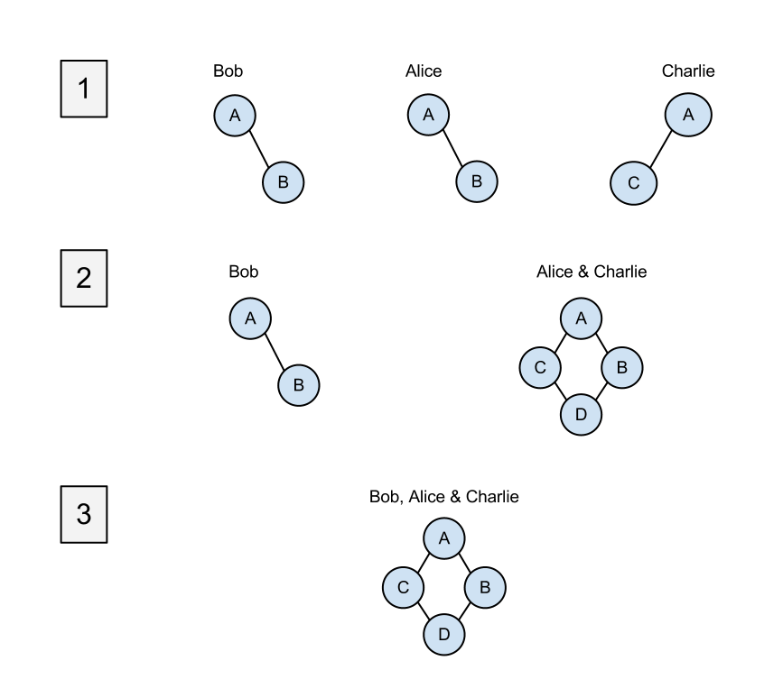
\includegraphics[width=5in]{image.png}
  \caption{Merge resolution for offline access.   \label{fig:image}}
\end{figure}

\vspace{5mm}
\noindent
\emph{One user, Alice, moves several paragraphs from one section of
  the paper to another, but does not change the contents of those
  paragraphs. Concurrently, another user, Bob, who is offline, edits a
  sentence in one of those paragraphs.}

\vspace{5mm}

When Alice and Bob meet, no conflict resolution will be
required. Alice's OTs are $X = move(12,422, 1022)$, etc.  The OT of
Bob's changes is $Y = insert(222, \text{``spurious text generation"})$. When Bob
meets Alice, his Collabrador client will synchronize with her, and
merge their text. The resulting transform will be 
\begin{equation*}
Y(X) \circ X = insert(822,
\text{``spurious text generation"}) \circ move(12,422, 1022)
\end{equation*}
The index 822 is determined as follows: index 1022 becomes index 612 because
\(1022-(422-12) = 612.\)  The original insert, at location 222, is 210
indices away from what is now index 612, and \(612+210 = 822.\) An equivalent
result can be achieved by
\begin{equation*}
X(Y) \circ X = move(12,448,1048) \circ insert(222, \text{``spurious text generation"})
\end{equation*}
where the \textit{new\_loc} and \textit{end\_index} have been incremented by 24 (the number of
characters in the inserted string).

\vspace{5mm}
\noindent
\emph{Two users, while not connected to each other, find a spelling
  mistake and correct the same word in the same way.}

\vspace{5mm}

Since the two versions have the same parent, change log and content,
the hashes will be the same, and they will be recognized as the same
version, making conflict resolution unnecessary.

\subsection{Failures}

Each Collabrador client keeps the list of users associated with a
document, and tracks whether or not they are reachable. A commit
cannot successfully begin unless all users are reachable. If any user
is disconnected during the commit process, the commit fails. The
commit may have created a node on some of the user' computers if it
partially completed. To avoid conflicts, Collabrador requires each
attempted commit to have a unique name. This ensures that no user will
ever have a commit with the same name in their DAG. If the commit
process notices that the commit name is already contained in a user's
DAG, the commit aborts immediately.

Synchronization can occur when a user's Collabrador client sees one or
more other users online, and it is a much more flexible process than
committing.  When user A decides to sync, a checkpoint is recorded to
the local graph.  If user A's machine crashes while saving the
checkpoint to the local graph, the checkpoint is lost
(all-or-nothing). If user A's machine crashes after saving the
checkpoint locally, but before initiating the sync process, then
Collabrador client will send out a sync request when user A comes back
online.  If user B crashes afterbeginning to send sync data to A, 
user A will terminate the sync process due to timeout and discard the
partial data. If any user goes offline after he finishes syncing with at least one
machine, but before all pairwise syncs have completed, the sync
process will go on amongst all other machines. The booted user will
re-synchronize during the integration process when he comes back
online.

We use TCP for reliable and accurate packet delivery, so we do not
have to worry about data corruption at the application layer. 

\subsection{Performance}

\subsubsection{Performance of the sync algorithm}

When two computers synchronize, the slowest step comes from
sending checkpoint databases from one computer to the
other. Recall that users are synchronizing continuously in
the background while connected to a network, so any
checkpoints saved while on the network will be synchronized
nearly immediately; in this case, the cost of a
synchronization is just the time it takes to send one
checkpoint from the provider to the initiator, and then one
more checkpoint (the merged document) from the initiator to
the provider.

In an ``average'' scenario, a user might click the ``save''
button (thereby creating a checkpoint) after typing a
paragraph. This document has paragraphs of 500--1000
characters each, so 1000 characters per checkpoint seems
reasonable. This corresponds to 1000 \emph{insert}
operations, each of which takes roughly 6 bytes to store (1
for the operation type, 1 for the character, and a 4-byte
integer for position). If the user made lots of edits,
there may also be about 1000 \emph{delete} operations, so
the entire OT would take 12,000 bytes. The other
information stored in the checkpoint object (e.g., the
parent hashes and user visibility list) are very small by
comparison. Thus, a normal checkpoint object appears to be
about 12 kilobytes, or roughly 100 kilobits. Over a 1
megabit per second Internet connection, this would take 0.1
seconds to transmit. As previously mentioned, the initiator
then needs to send a checkpoint back to the provider, so a
sync step might take 0.2 seconds total.

If a user goes offline for some time and then attempts to
sync, the synchronization will take considerably longer
because it needs to transmit information about \emph{all}
checkpoints that occurred while the user was offline.
Assuming (as before) that the space for storing the OT is
the costliest requirement, it is sufficient to consider how
large an OT may be after a user has been offline for a
while. Consider, for instance, what happens if a user
writes an entire 5,000-word paper while offline and then
attempts to sync. In this paper, each word is about 10
characters, so the edit would be roughly 50,000 characters.
If the user went through many revisions while offline,
there may be lots of deletions per inserted character. For
lack of good data on how much overhead this would impose,
make the assumption that this adds an order of magnitude of
overhead, so there are 500,000 OT operations. Each one
takes 6 bytes, so the overall data that needs to be
transferred is 3 megabytes (or 24 megabits). This would
take 24 seconds!

At first glance, it may seem like this 24-second operation
would be prohibitively expensive in a network with many
computers. Consider for example a network with 10 users. If
a user $A$ who has been offline for a while comes online,
it would take 240 seconds (or 4 minutes) for user $A$ to
communicate with all other users. However, once a user $B$
knows about $A$'s edits, user $B$ can also send those edits
to others through the sync process. The spread of $A$'s
edits in the system will follow a logistic curve, so
propagating $A$'s edits to all users will only take
logarithmic (rather than linear) time in the number of
users.

\subsubsection{Performance of the merge algorithm}

The time taken by the merge algorithm grows linearly with the number
of changes between the two leaves and their lowest common ancestor.
Assuming that it takes a thousand CPU cycles to process a single OT
primitive, the process of merging two encyclopedias would take less
than a millisecond.  Thus, we are not especially concerned with
performance of the OT merge algorithm.  (Moreover, the time taken by
the merge algorithm is negligible compared to the time taken by a user
to manually resolve a conflict.)

Using the naive approach, opening a merged DAG for editing takes
linear time in the size of the document history, since the complete
set of OTs must be layered upon the root of the DAG.  This can be
mitigated by caching file contents for each node in the DAG, and
selectively reordering OTs to minimize the number of primitives
required to represent each operation.

\subsection{Design Tradeoffs and Flaws}

Having no centralized server makes Collabrador a more reliable
document editing system, because there is no single point of
failure. It also allows for increased flexibility, as users can edit
while connected to the internet, ad-hoc, or offline. However, because
Collabrador is distributed, synchronizations are pairwise, making the
sync algorithm quadratic with respect to the number of users. A
centralized server would have asymptotically linear synchronization.

Some collaborative editors use version vectors: a vector containing
the last known version number for each user. For example, \(V = (1, 2,
2)\) means that the first user has version 1 of the document, and the
other two have the second version.  This is a compact and nifty way to
represent version data. \(V_1\) is newer than \(V_2\) if all of
\(V_1\)'s elements are greater than or equal to \(V_2\)'s. If one
vector is not clearly older than another, e.g. \(V_1 = (1,2,3)\) and
\(V_2 = (3,1,4)\), then there is a conflict. A DAG is more visually
informative than a version vector and provides an intuitive way for
users to visually track the document history. The DAG allows us to
perform OTs and use a highly autonomous merge algorithm.  A system
using version vectors would require the user to merge conflicts more
frequently, since less information is available. The cost, however, is
that the DAG grows linearly with edit history. The more frequently a
document has been committed, the more overhead there is. Version
vector overhead only increases as the number of users editing a
document increases.

We support only named checkpoints or dynamic membership, not
both. This is because the ability to delete users greatly complicates
things. For example, if user A is deleted, and broadcasts while only
user B is available, but then user B is deleted before he can pass on
the word about user A. This presents problems for commits, because all
users are required to be online.  Also, if a user were allowed to join
while a commit was underway, the initiator might receive a visibility
list that does not include the new user, and think that it is correct
because his client was unaware of the new user.  There are ways around
these problems, but this is a challenge we have left for later
releases. The feature was not included in the first release because
static groups greatly simplify the design, and allows Collabrador to 
have stronger guarantees about correctness.

Finally, it is worth noting that Collabrador does not have an
authentication system, so it is very simple for a user to send false
changes.

\section{Conclusion}

Collabrador is a sophisticated collaborative document editing system
that gives users flexibility in connectivity. It uses
industry-standard operational transforms to merge changes, and has a
failure-resistant synchronization process.  Problems that remain to be
solved include dynamic membership and adding an authentication system.

\bibliographystyle{IEEEtran} \bibliography{IEEEabrv,dp2}

4832 words

\end{document}
